\section{Simulação}

\subsection{Modelo do Sistema Elétrico}

\subsubsection{Sistema de Geração} \todo{falar da potência do gerador}

O sistema de geração aplicado na simulação visa representar de maneira suficientemente apropriada uma fonte de tensão comumente encontrada em sistemas elétricos aeronáuticos. Tal bloco é composto por uma máquina síncrona, cuja entrada mecânica é definida por um valor constante representado pela rotação do eixo proveniente do IDG, e os níveis de tensão é determinado por controle de campo de excitação. Esse último é obtido por uma GCU a qual opera juntamente com a maquina síncrona do gerador. Em sistema elétricos aeronáuticos reais a complexidade do bloco Gerador/GCU é complexa e envolve sistemas complementares para garantir sua confiabilidade. Entretanto, para a proposta de simulação apresentado nesse trabalho, o sistema proposto por \cite{Olivier} mostra-se adequado. Isto deve-se principalmente pela característica da saída do gerador apresentar tensão com certa frequência definida, com amplitude controlada e as não idealidades representadas pelas resistências e indutâncias nas linhas do gerador são modeladas.

Em ambiente Simulink tanto o bloco da máquina síncrona como o bloco de excitação de campo estão presentes. Sendo assim o sistema de geração utilizado no software é mostrado na Figura \ref{fig:GEN_GCU.png}.

\begin{figure}[!htb] %
	\centering
	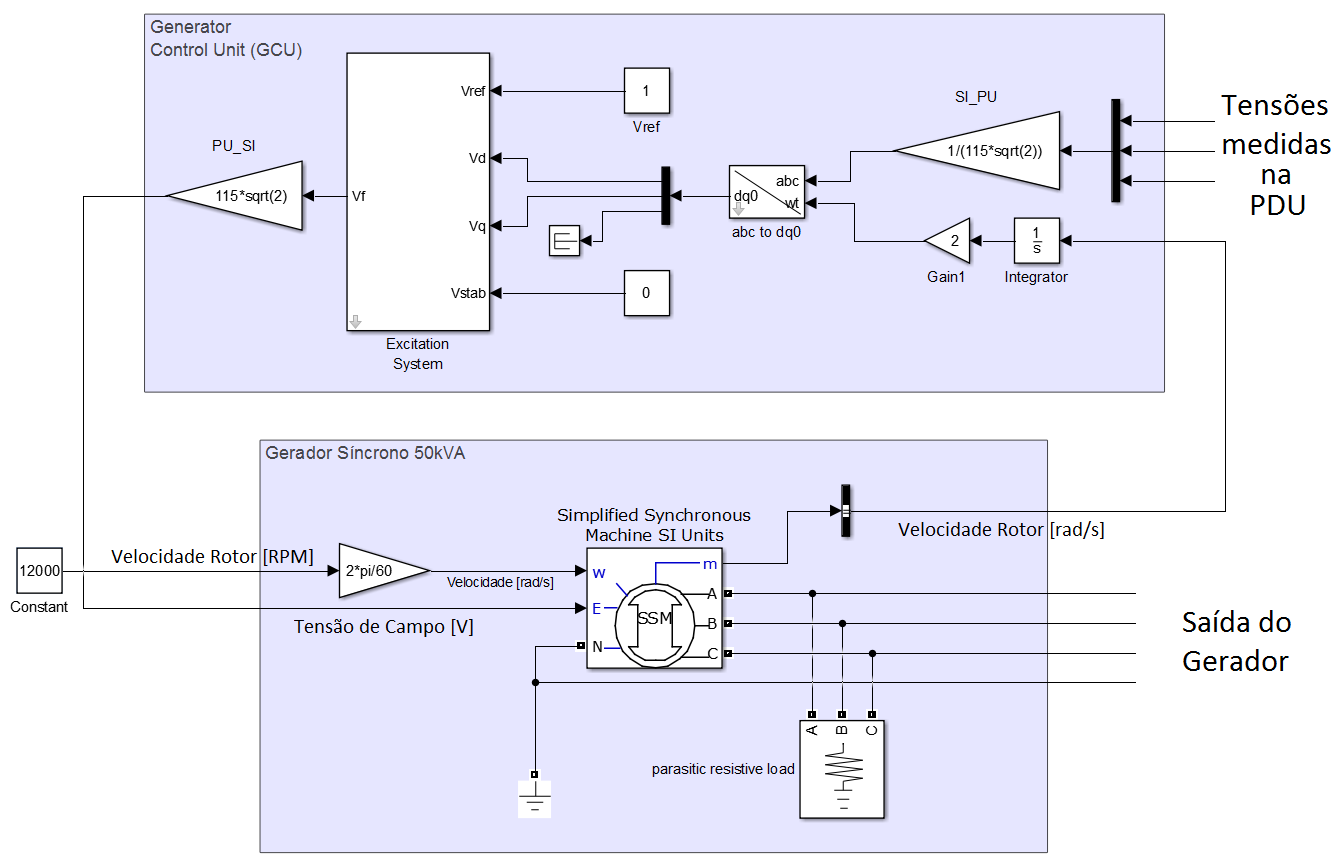
\includegraphics[width=0.99\textwidth]{Cap4/Figuras/GEN_GCU.png}
	\caption{Modelo do sistema de geração}
	\label{fig:GEN_GCU.png}
\end{figure}

Nessa ilustração o subconjunto superior é composto pelos elementos que modelam a GCU. O \textit{Excitation System} é um bloco nativo do Simulink, a qual opera como descrito em \cite{IEEE}. Já os blocos auxiliares da GCU estão presentes para condicionar o sinal adequadamente. A medição de tensão que alimenta a GCU deve ser proveniente do barramento de distribuição, visto que as não idealidades do sistema alterem os níveis de tensão nesse ponto em comparação à saída do gerador.

O subconjunto inferior compõe o Gerador. A máquina síncrona é também um bloco presente no Simulink e em sua saída estão presentes as resistências e indutâncias conectadas em série, cujos valores são expostos na Tabela \ref{tab:Zgen}.  Ainda existe uma resistência parasita no sistema com o intuito de evitar problemas numéricos na simulação. A presença deste elemento não influencia o sistema que será simulado.

\begin{table}[!htb]
	\centering
	\begin{tabular}{|c|c|c|}
		\hline
		\textbf{Resistência	[$\Omega$]}	& \textbf{Indutância [mH]}	& \textbf{Impedância (400 Hz) [$\Omega$]}\\\hline
		0.0404					& 0.09204			& $0.0404+j0.213$\\
		\hline
	\end{tabular}
	\caption{Impedância interna do Gerador}
	\label{tab:Zgen}
\end{table}

\subsubsection{Sistema de Distribuição}

O sistema de distribuição de uma aeronave é constituído pelos condutores que transferem a energia entre os subsistemas, além dos barramentos de distribuição e equipamentos de proteção do sistema elétrico. Contudo, nesse trabalho as proteções não estão no escopo da simulação, sendo que o modelo proposto será composto apenas pelas linhas de transmissão e um barramento a qual as cargas possam ser conectadas.

O ponto de conexão em comum está localizado na PDU (\textit{Primary Distribution Unit}). Apenas um barramento será considerado e as cargas não lineares compostas pelos EHAs serão conetadas em paralelo a partir dessa unidade. A Figura \ref{fig:dist.png} apresenta o modelo implementado no Simulink para realização da simulação. Aqui pode-se observar as cargas compostas pelos EHAs sendo conectadas a partir da PDU. A alimentação da PDU é realizada diretamente pelo gerador através de uma linha de transmissão trifásica. Nessa unidade ainda existe um sensor de tensão que cede informação ao GCU para o controle de excitação de campo, a qual fornecer ao gerador o controle para que este apresente níveis de tensão adequadas para manter a tensão de fase no PCC sendo 115 V.

\begin{figure}[!htb] %
	\centering
	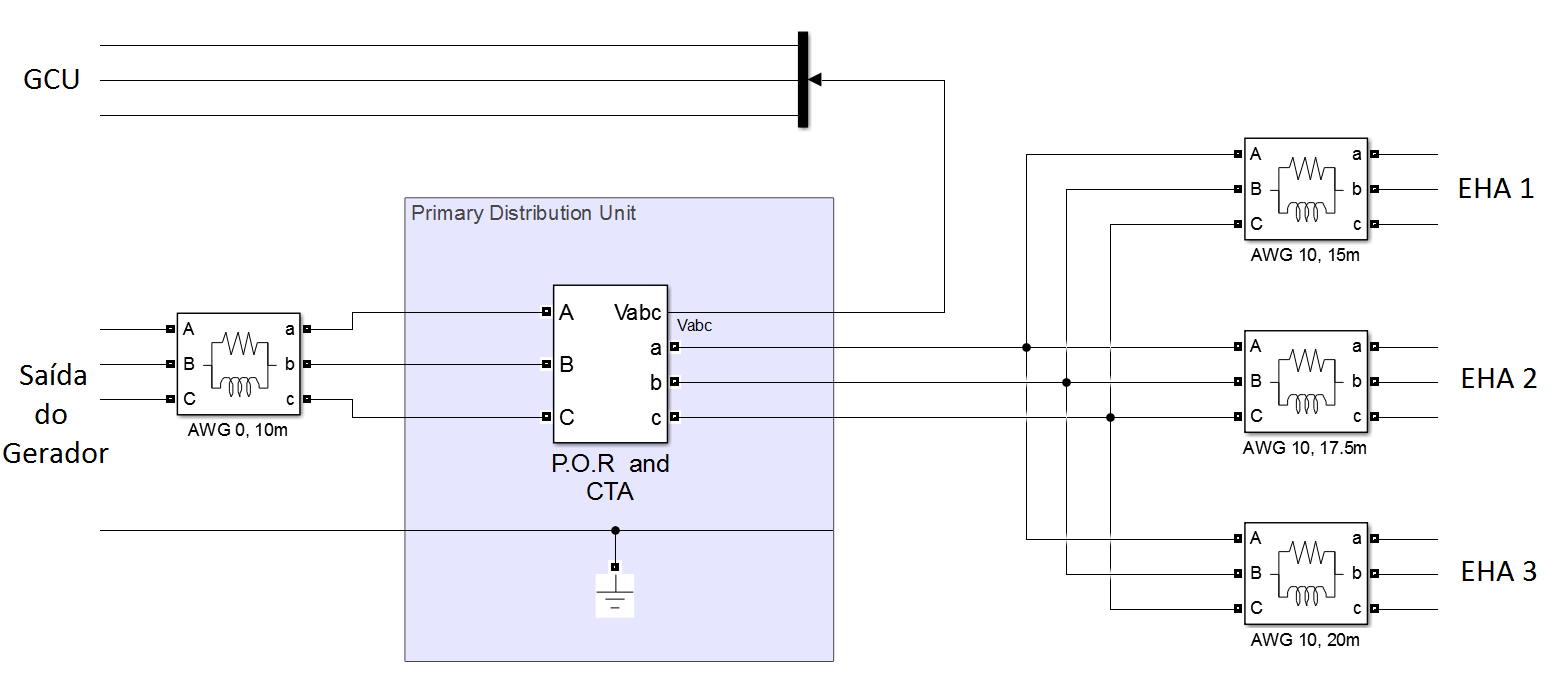
\includegraphics[width=0.99\textwidth]{Cap4/Figuras/dist.png}
	\caption{Sistema de Distribuição}
	\label{fig:dist.png}
\end{figure}

As não idealidades dos condutores são modeladas com a inserção de resistências e reatâncias indutivas conectadas em série nas linhas de transmissão do sistema. As capacitâncias entre os condutores e o plano de terra não são considerados devido sua insignificância frente a potência e o tamanho das cablagens. As bitolas dos fios e seus comprimentos estão adequadamente dimensionados para a corrente transmitida e o tamanho comumente encontrado em uma aeronave do porte do modelo, respectivamente. Sendo assim, os valores de impedância de cada seção do sistema trifásico é definido seguindo os parâmetros encontrados em \cite{Exner1953}. A Tabela \ref{tab:Zdist} expõe as definições do modelo quanto às cablagens utilizadas e suas impedâncias de cada seção. 

\begin{table}[!htb]
	\centering
	\begin{tabular}{|c|c|c|c|}
		\hline
		\textbf{Porção}		&	\textbf{Bitola}		&	\textbf{Comprimento}	&	\textbf{Impedância (400 Hz) [$\Omega$]}	\\\hline
		GEN - PDU	&	AWG 0		&	10 m		&	$0,0047+j0,0067$	\\\hline
		PDU - EHA 1	&	AWG 10 		&	15 m		&	$0,0540+j0,0199$	\\\hline
		PDU - EHA 2 &	AWG 10		&	17.5 m 		&	$0,0630+j0,0233$	\\\hline
		PDU - EHA 3	&	AWG 10		&	20 m 		&	$0,0720+j0,0266$	\\\hline
	\end{tabular}
	\caption{Impedâncias das linhas de distribuição}
	\label{tab:Zdist}
\end{table}

\subsubsection{Atuador Eletrohidrostático}

O atuador eletrohidrostático é um dispositivo empregado em sistemas de controle de voo na qual atua nas superfícies de comando para manter a aeronavegabilidade de uma aeronave. Os EHAs são compostos por dois principais subsistemas: o subsistema elétrico e o subsistema hidráulico. A porção elétrica é composto por conversores de tensão elétrica de modo a energizar um motor que impulsiona a bomba do subsistema hidráulico. Com a pressurização das linhas hidráulicas o EHA fica apto a acionar o deslocamento linear do pistão por meio da atuação de sistemas de controle.

A subsistema elétrico tem como principais componentes uma ponte trifásica de diodos, um driver DC-DC, um inversor de frequência e uma máquina síncrona baseada em imãs permanentes \cite{Dinca2014}. A Figura \ref{fig:EHA_elec.png} mostra o diagrama simplificado do subsistema elétrico. Cabe lembrar que outros componentes secundários são empregados neste subsistema com o intuito de prover controle e proteção ao EHA, e que não são mostrados na Figura \ref{fig:EHA_elec.png}.

\begin{figure}[!htb] %
	\centering
	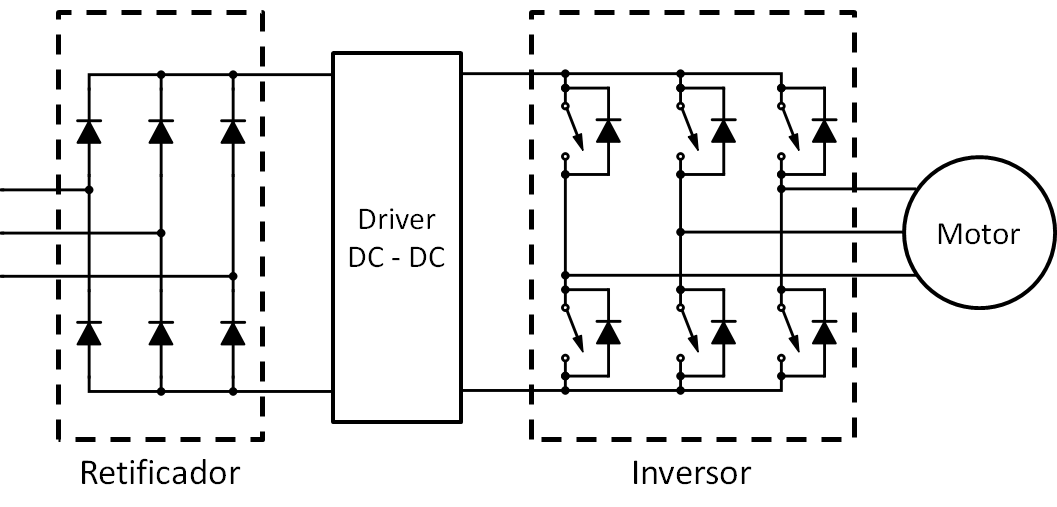
\includegraphics[width=0.7\textwidth]{Cap4/Figuras/EHA_elec.png}
	\caption{Subsistema elétrico de um EHA}
	\label{fig:EHA_elec.png}
\end{figure}  

Por apresentar uma ponte de retificadora de diodos na entrada, a operação de um EHA acaba por injetar componentes harmônicas nas formas de onda de corrente, trazendo assim a depreciação da qualidade de energia elétrica de uma aeronave. Como o foco deste trabalho diz respeito à qualidade de energia, tanto a modelagem do subsistema hidráulico juntamente com a operação do motor elétrico não serão modelados. Sendo assim, o foco recai nas formas de onda da corrente que atravessam o retificador de entrada, a qual é o principal componente responsável pela queda na qualidade de energia quando se opera o EHA. A Figura \ref{fig:EHA.png} mostra o modelo do EHA empregado no Simulink para realização da simulação. Este modelo é composto por uma ponte retificadora trifásica que interfaceia a conversão AC-DC, como em um EHA, sendo que no lado DC exite uma fonte de corrente controlada. A realização desta fonte tem por objetivo simular o comportamento de consumo de energia proferido pelo restante dos componentes do lado DC do subsistema elétrico. A presença de uma resistência \textit{snubber} em paralelo à fonte de corrente tem como objetivo eliminar incompatibilidades do modelo, visto que isto é uma exigência para compilação do Simulink. Contudo, o valor de $R$ é escolhido com alto valor de resistência de maneira que este interfere insignificantemente ao sistema.

\begin{figure}[!htb] %
	\centering
	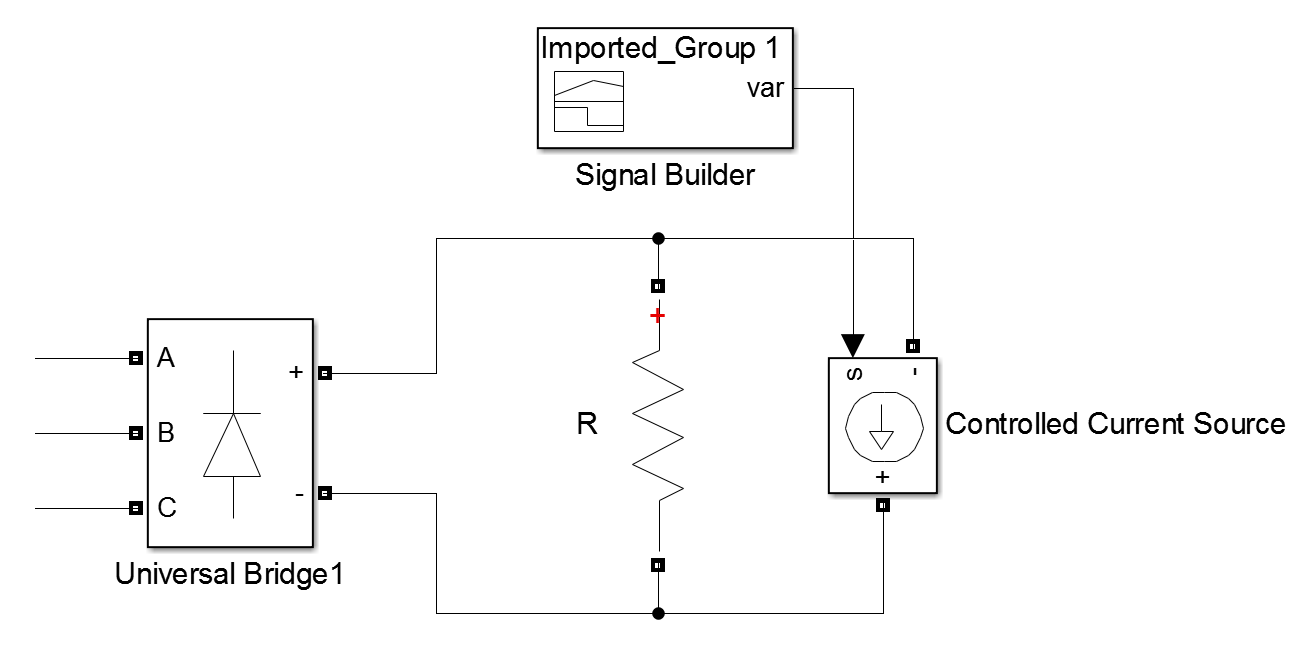
\includegraphics[width=0.7\textwidth]{Cap4/Figuras/EHA.png}
	\caption{Modelo do EHA empregado no Simulink}
	\label{fig:EHA.png}
\end{figure}

O sinal de controle da fonte de corrente do lado DC é realizado de maneira a providenciar adequadamente o consumo de corrente visto pelo lado AC de um EHA. Tal sinal de controle foi gerado utilizando resultados experimentais de um EHA operando com carga em seu pistão. A metodologia empregada para a obtenção do sinal de controle da fonte de corrente foi através do cálculo da potência aparente consumida de um EHA real, através de dados experimentais, e inferir essa mesma potência no lado DC do EHA do modelo. Com isso garante-se que a potência aparente apresentada no modelo seja a mesma de um EHA real operando com carga, além de garantir a equivalência das formas de onda da corrente no lado AC. Com essa metodologia empregada o sinal criado para o controle da fonte de corrente do lado DC do modelo é visto na Figura \ref{fig:corrente_controlada_EHA.eps}.

\begin{figure}[!htb] %
	\centering
	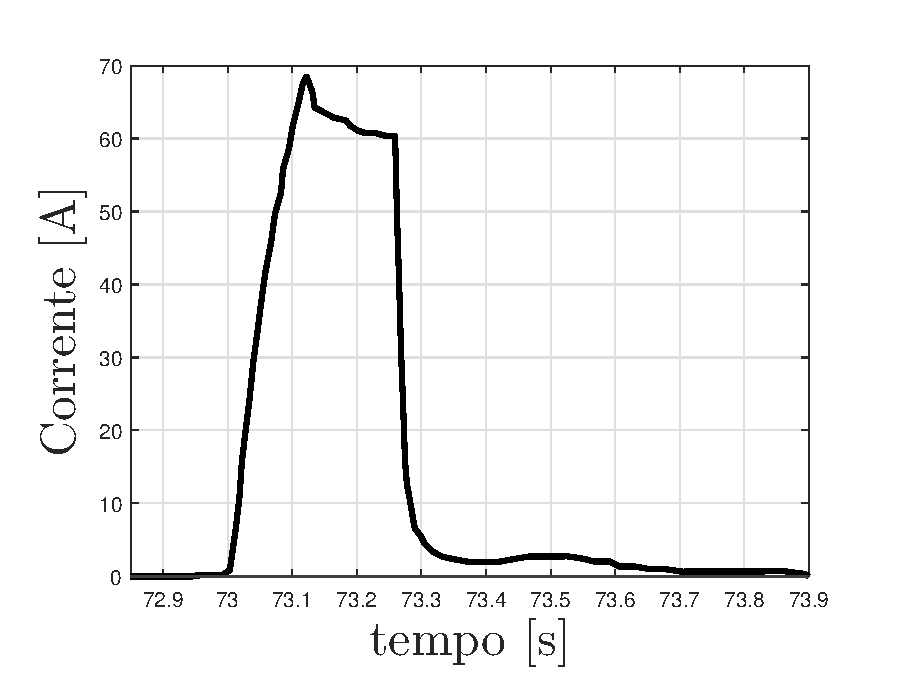
\includegraphics[width=0.7\textwidth]{Cap4/Figuras/corrente_controlada_EHA.eps}
	\caption{Valores estipulados na fonte de corrente controlada}
	\label{fig:corrente_controlada_EHA.eps}
\end{figure}

\todo{Padronizar as figuras (plots\_EHA\_teste.mat)}

\subsection{Modelo do Filtro Ativo}

O filtro ativo modelado em ambiente Simulink tem como objetivo simular a operação do controle do compensador de maneira suficientemente adequada para avaliar a eficácia da filtragem e seu emprego no setor aeronáutico. Com isso, as diversas características que viabilizam o emprego desse tipo de filtro podem ser analisadas.

O modelo é composto por diversos bloco criados para cada função constituinte de um filtro. As teorias de potência instantânea apresentadas no capítulo \ref{cap:Filtros Ativos para Sistemas Elétricos} serão implementadas em um desses blocos para realizar a simulação dos cálculo das correntes de referências do compensador. Já a parte relacionada com o compensador será implementado em outro bloco e segundo as definições apresentadas na seção \ref{sec:Características de Filtros Ativos em Sistemas Reais}. A operação conjunta do compensador com o controle concebe o filtro ativo como todo.

\subsubsection{Controle}

O bloco de controle visa simular os procedimentos de cálculo, os comandos dos interruptores estáticos do compensador e a malha de controle de tensão do capacitor do lado DC do inversor. Estes sub-blocos são comumente encontrados em dispositivos programáveis de sistemas reais as quais compõem o DSP.

O sub-bloco de cálculo das correntes de referência para o inversor é mostrado na figura \ref{fig:controladador.png}. Este sub-bloco tem como entrada as tensões medidas nas linhas trifásicas do sistema elétrico no ponto anterior a conexão do filtro, e também, as correntes medidas na entrada da carga não linear, onde no caso dessa simulação é dada pelo EHA. Já a saída é composta pelas correntes de referência que alimentam o controle de comando dos interruptores do inversor estático.

O sub-bloco a qual determina as correntes de referência é constituído de duas partes, onde a porção superior da figura \ref{fig:controladador.png} compõe o detector de sequencia positiva, e a parte inferior constitui o cálculo das correntes de referência. A porção superior utiliza a teoria apresentada na seção \ref{subsubsec:Tipos de Controle} e estabelece os cálculos algébricos para a obtenção do sinal das tensões sem apresentar harmônicas ou componentes de sequência negativa ou zero. Este sinal é direcionado para a porção inferior, onde utiliza-o juntamente com as equações da teoria da potência instantânea, a qual são extensamente discutidos no capítulo \ref{cap:Filtros Ativos para Sistemas Elétricos}, para  a obtenção das correntes de referência do filtro.

\begin{figure}[!htb] %
	\centering
	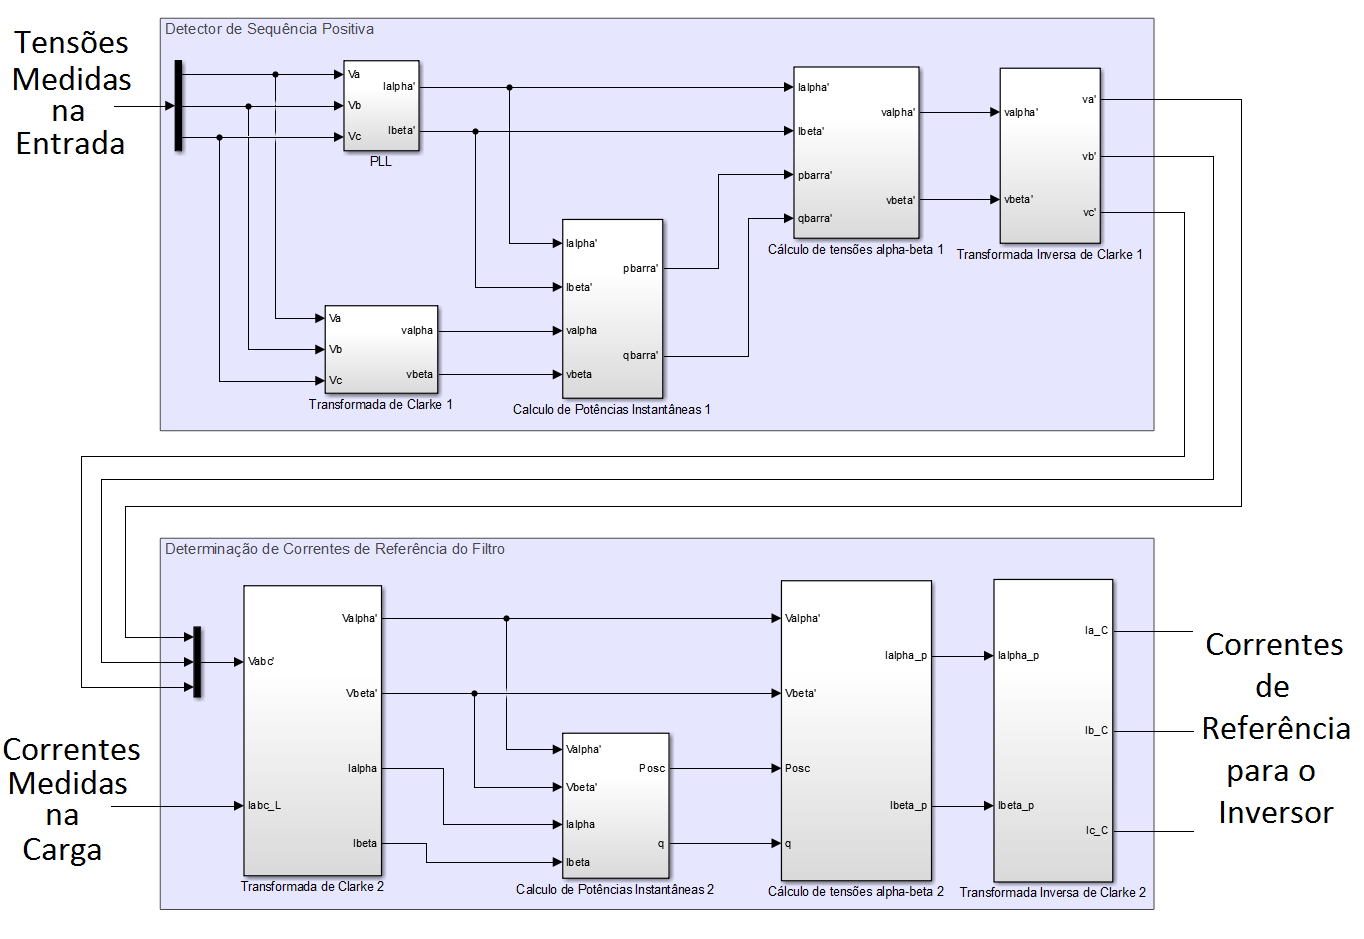
\includegraphics[width=0.99\textwidth]{Cap4/Figuras/controlador.png}
	\caption{Sub-bloco para determinação das corrente de referência}
	\label{fig:controladador.png}
\end{figure}

O sub-bloco de comando dos interruptores estáticos do inversor, onde é empregado o controle por histerese, é mostrado na Figura \ref{fig:histerese_sim.png}. Nesse bloco a entrada é composta pelos sinais de referência das correntes advindas do sub-bloco da Figura \ref{fig:controladador.png} (I\_ref), juntamente com a medição da corrente na saída do inversor (I\_meas). A saída é composta pelo sinal de comando de cada interruptor a qual é empregado no inversor.

A operação deste bloco é realizada pela comparação do sinal de referência com a medição da corrente na saída do inversor. O sinal advindo da comparação passa por um relé programado com histerese, onde é definida a banda de histerese, e por fim a saída contendo um sinal binário é gerado. Os sinais de cada fase do sistema é gerado individualmente com o controle de comutação dos interruptores de cada braço do inversor. Como estes interruptores não podem ser comutados para o estado de condução simultaneamente, seus comandos devem ser complementares. Este complemento é adquirido pela função NOT do sub-bloco.

\begin{figure}[!htb] %
	\centering
	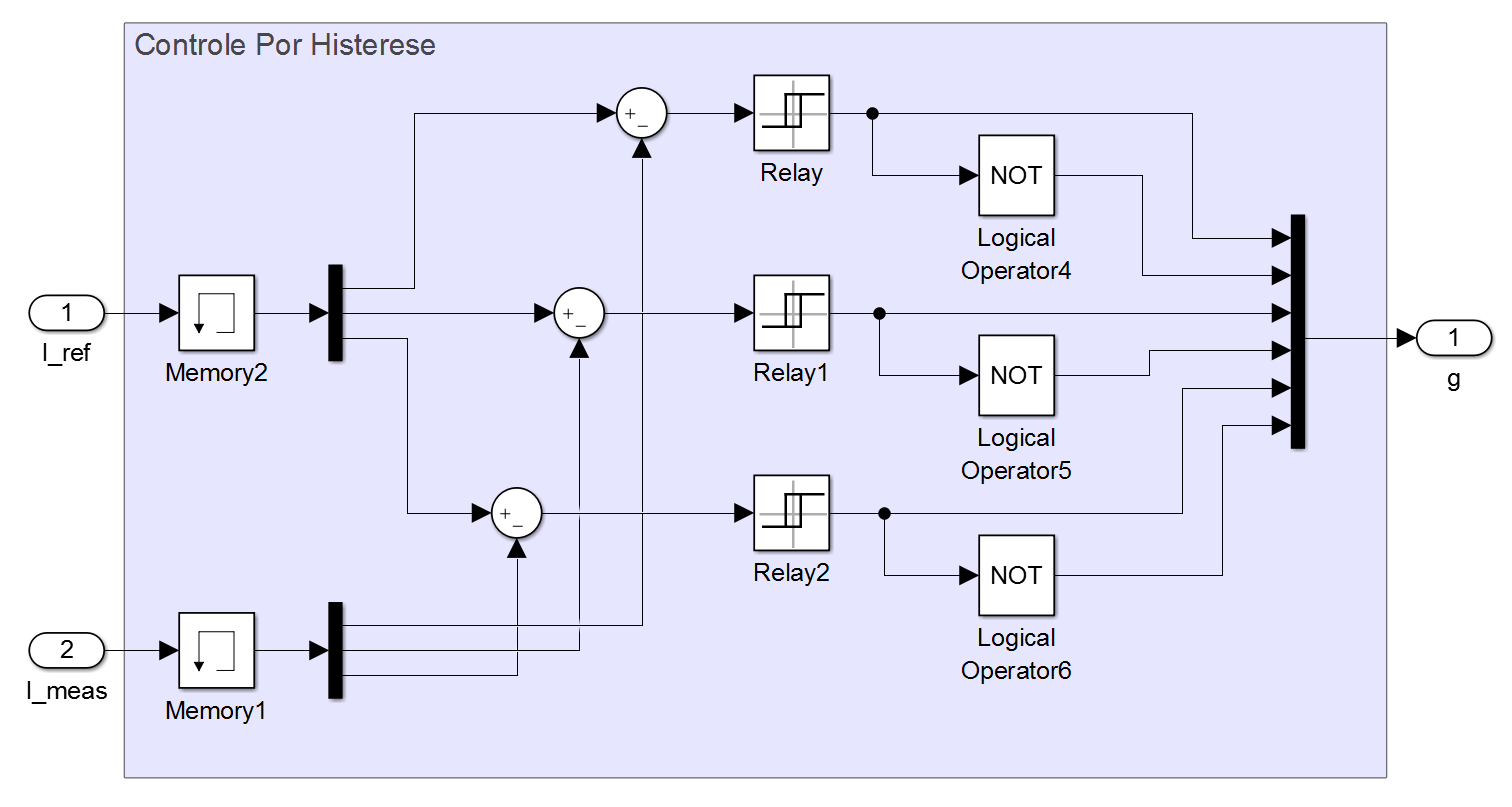
\includegraphics[width=0.7\textwidth]{Cap4/Figuras/histerese_sim.png}
	\caption{Obtenção do sinal de comando dos interruptores por controle de histerese}
	\label{fig:histerese_sim.png}
\end{figure}

O controle de tensão do capacitor disposto no lado DC do inversor é mostrado na Figura \ref{fig:PI_sim.png}. Este sub-bloco tem em sua entrada a medição de tensão do capacitor, ao passo que em sua saída é disponibilizado o sinal de potência das perdas acorridas na operação do inversor. Tal sinal de saída é direcionado para calculo das potências instantâneas do sub-bloco de determinação de correntes de referência (Figra \ref{fig:controladador.png}).

Este bloco constitui de um controlador proporcional-integral (PI), onde os valores de $P$ e $I$ são escolhidos de maneira a apresentar uma resposta do controlador adequada o funcionamento do sistema. A referência é obtida como um sinal degrau com amplitude fixa e início definido no tempo para evitar o transitório do sistema de geração, a qual pode gerar instabilidade numérica do Simulink. 

\begin{figure}[!htb] %
	\centering
	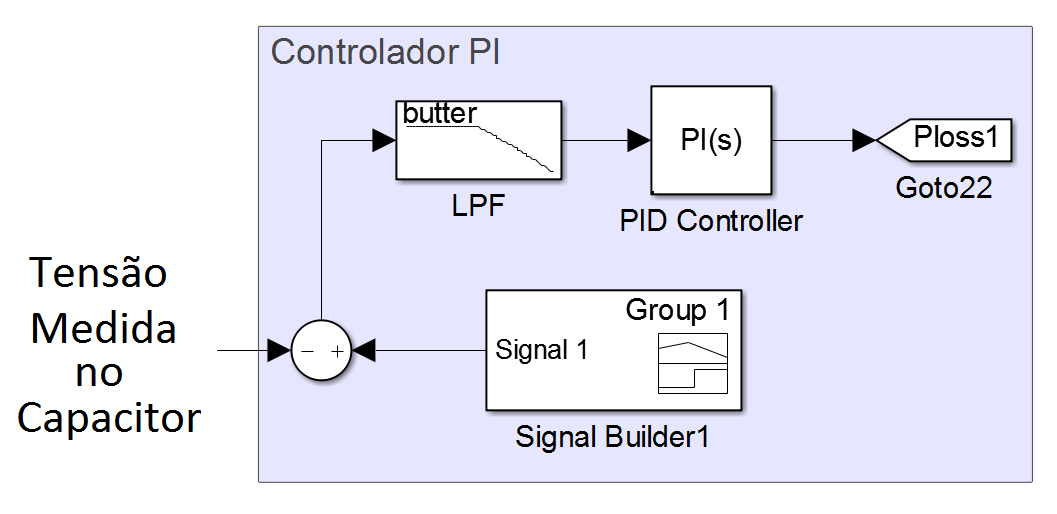
\includegraphics[width=0.5\textwidth]{Cap4/Figuras/PI_sim.png}
	\caption{Valores estipulados na fonte de corrente controlada}
	\label{fig:PI_sim.png}
\end{figure}

\subsubsection{Compensador}

O compensador criado em ambiente Simulink tem como objetivo simular a operação de um inversor composto por interruptores estáticos, nas quais são controlados pelos sinais gerados no bloco de controle para atender a demanda de corrente necessária para realização da filtragem ativa. Este bloco tem como entrada os sinais de comando dos interruptores advindos do bloco de controle por histeres. Ainda, para a correta operação do compensador algumas medições são realizadas para realimentar o bloco de controle. Com isso, a forma de onda da corrente na saída do compensador é adquirida para realimentar o sub-bloco de controle por histerese e a tensão no capacitor é medida para prover informação ao sub-bloco de malha de controle de tensão no capacitor. Em sua saída o compensador é conectado no barramento de alimentação na entrada da carga não linear conecatda na rede elétrica da aeronave.

A Figura \ref{fig:Inversor.png} apresenta o bloco do compensdor utilizado na simulação. Nesse bloco é utilizado uma ponde de interruptores estárticos ideais ordenadado como ilustrado na Figura \ref{fig}. A escolha dos interrupotres serem estabelecidos como ideais recai na limitação do Simulink com relação às não idealidade apresentadas em elementos semicondutroes de comutação.
 
\begin{figure}[!htb] %
	\centering
	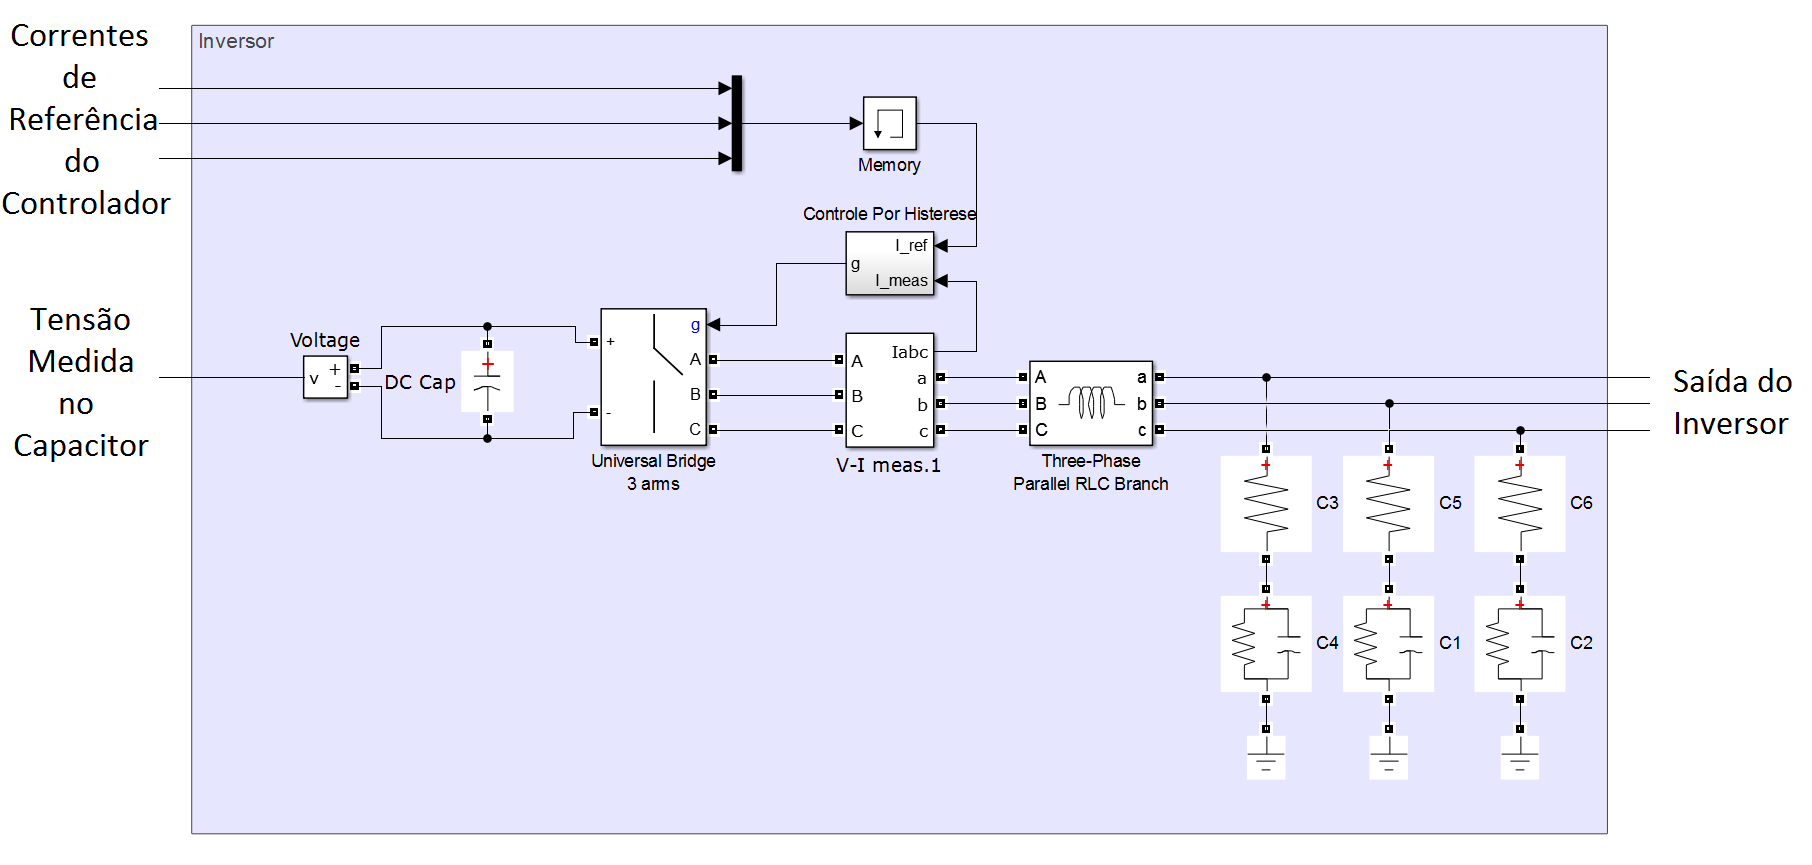
\includegraphics[width=0.99\textwidth]{Cap4/Figuras/Inversor.png}
	\caption{Valores estipulados na fonte de corrente controlada}
	\label{fig:Inversor.png}
\end{figure}

\subsection{Resultados}
